\chapter[Implementazione]{Implementazione}
\label{chap:Implementazione}
Il software si pone l'obiettivo di verificare se un programma, composto da una o più query e da codice che ne usa i risultati, sia corretto o meno. Per le query si tratta di verificare se essa sia abitata o meno. Per quanto riguarda invece l'uso dei risultati si tratta di verificare se sia ben tipato o meno. Da queste due responsabilità abbiamo derivato due moduli: un modulo Reasoner, scritto in java che si occupa di determinare l'abitabilità delle query, e un modulo scritto in OCaml che si occupa di tipare il programma.

\section{Il linguaggio $\boldsymbol{\lambda_{DL}}$}
    Quando si effettua una computazione basata su ontologie, il processo di ragionamento è portato avanti a run time, e se si scoprono assiomi non soddisfacibili 
    il programma potrebbe essere soggetto a errori. Non è quindi possibile garantire che un'esecuzione termini correttamente, ovvero si otterrà il risultato aspettato. 
    Il nostro obiettivo è quello riuscire a catturare questi errori prima dell'esecuzione, andando ad assicurare una computazione senza errori run-time che dipendono dalla base di conoscenza. 
    Vorremmo quindi valutare vantaggi e efficienza di un controllo statico, sfruttando i sistemi di tipi per assicurare la correttezza statica del programma, rispetto a 
    un'ontologia basata sulle logiche descrittive (in particolare OWL). Sforzi verso questa direzioni sono stati già proposti nella tesi di dottorato di Martin Leinberger, 
    in cui propone un lambda calcolo tipato esteso con interrogazioni SPARQL a basi di triple RDF e costrutti della logica descrittiva come tipi chiamato $\lambda_{DL}$.
    \\ Il linguaggio garantisce di eseguire delle QUERY SPARQL che rispettano A-Box e T-Box dell'ontologia, spostando il controllo dell'abitabilità durante il type checking e
    permettendo di tipare i nodi ritornati dalle Query tramite le concept expressions della logica descrittiva.
    L'esempio successivo, preso dalla tesi di Leinberger, mostra un programma scritto in $\lambda_{DL}$ che espone chiaramente le potenzialità del linguaggio.
    \begin{figure}[h]
        \captionsetup{singlelinecheck = false}
        $K_4 = $\{Students $\sqsubseteq$ Person
        \\Professor $\sqsubseteq$ Person\}
        \begin{minted}[escapeinside=||,mathescape=true, autogobble]{ocaml}
            (head (query x |$\leftarrow$| x type Student)).x
        \end{minted}
        \caption{Programma in $\lambda_{DL}$ avente come knowledge base $K_4$}
    \end{figure}
    \\Il programma esegue una query SPARQL che ritorna una lista di mapping tra la variabile \textbf{x} e nodi del grafo RDF che rispettino il vincolo
    \textbf{x type Students}. Successivamente prendiamo il primo elemento della lista (\textbf{head}) e lo proiettiamo sulla variabile \textbf{x} (\textbf{(...).x}).
    Il sistema di tipo ci permette di:
    \begin{itemize}
        \item stabilire la correttezza della query, costruendo degli assiomi dalla sua struttura e richiamando un reasoner.
        \item dare un tipo ai nodi ritornati dalla query. Nel nostro esempio tutta l'espressione è di tipo \textbf{Students} e grazie al subtyping e al fatto
            che nella knowledge base sappiamo che Students $\sqsubseteq$ Person è anche ti tipo \textbf{Person}.
    \end{itemize}
    L'implementazione si concentra solo sul type system, i riferimenti agli aspetti più teorici del linguaggio insieme alla sintassi e le regole di valutazione
    si possono trovare nella tesi di Leiberger.
    Vale la pena per\`o accennare che il linguaggio è corretto, ovvero un termine chiuso e ben tipato non si blocca durante la valutazione.
    La corretteza è dimostrata da Leinberger attraverso due teoremi:
    \begin{theorem}
        (Progress in $\lambda_{DL}$): sia t un termine ben tipato e chiuso. se t non è un valore, allora esiste una termine t' tale che
        t $\xrightarrow[]{\text{K}}$ t'. Se $\Gamma$, K $\vdash$ t : T, allora t è un valore o un termine contenente head nil[T] e tail nil[T] oppure esiste
        un t' per cui t $\xrightarrow[]{\text{K}}$ t'
    \end{theorem}
    \begin{theorem}
        (Preservation in $\lambda_{DL}$): Sia t un termine e T un tipo. Se un tipo è assegnato a t, scritto $\Gamma,K \vdash t : T$ e t $\xrightarrow[]{\text{K}}$ t'
        allora, $\Gamma,K \vdash t' : T$
    \end{theorem}
    Entrambe le dimostrazioni sono per induzione su $\Gamma,K \vdash t : T$ e i dettagli si possono trovare nella tesi di Leinberger.

\newpage
\section{OCaml Module - Le query}
L'idea alla base del modulo OCaml è la seguente:
\begin{enumerate}
    \item la query in formato testuale viene parsificata in un tipo Query
    \item sul tipo Query vengono inferiti gli assiomi di Leinberger
    \item viene invocato il Reasoner e gli vengono passati gli assiomi appena inferiti.
    \item il risultato del Reasoner viene raccolto dal modulo OCaml
\end{enumerate}
Vediamo questi passaggi nel dettaglio

\subsection{Parsificazione}
Per generare il parser, ho utilizzato il programma OCamlyacc, un compilatore di compilatori per OCaml, ispirandomi alla grammatica delle query SPARQL\ref{fig:leinbergerSyntax}.
Per definire i token che compongono la grammatica invece mi sono avvalso di OCamllex, un generatore di lexer.

Il parsificatore così generato ha la responsabilità di riconoscere se la query rispetta la grammatica\ref{fig:leinbergerSyntax}. Se cosi è, allora viene generato un tipo Query\ref{fig:querType}, che racchiude tutte le informazioni presenti all'interno della query in formato testuale.

\begin{figure}[H]
    \centering
    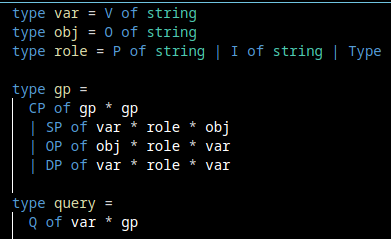
\includegraphics[scale=0.7]{pictures/queryType.png}
    \caption{tipo Query corrispondente alla sintassi delle query SPARQL CQ}
    \label{fig:querType}
\end{figure}


Per esempio, data questa query di input:

\begin{minted}[escapeinside=||,mathescape=true, autogobble]{ocaml}
 query x <- (x type Pizza AND x hasTopping y AND y type GorgonzolaTopping)
\end{minted}

otteniamo il seguente tipo Query così costruito:

\begin{minted}[escapeinside=||,mathescape=true, autogobble, breaklines, linenos]{ocaml}
Q (V x, CP (SP (V x, TYPE, Pizza), CP (DP (x, P hasTopping, y), SP (y, TYPE, P GorgonzolaTopping))))
\end{minted}

\subsection{Inferenza degli assiomi di Leinberger}
Introduciamo il tipo ClassExpression, definito ispirandosi alle regole di derivazione degli assiomi di Leiberger, che servirà per generare gli assiomi di Leinberger.
\begin{figure}[H]
    \centering
    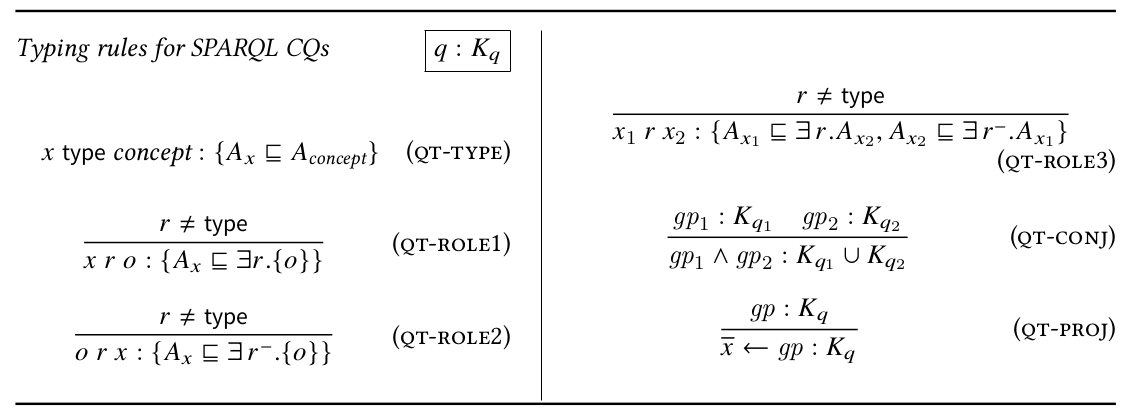
\includegraphics[width=\textwidth]{pictures/leinbergAxiom.png}
    \caption{Regole di derivazione degli assiomi di Leiberger}
    \label{fig:leinbergerAxiom}
\end{figure}

\begin{figure}[H]
    \centering
    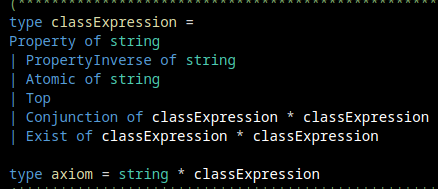
\includegraphics[width=\textwidth]{pictures/classExpressionType.png}
    \caption{Il tipo ClassExpression e Axiom}
    \label{fig:enter-label}
\end{figure}
Gli assiomi di Leinberger vengono inferiti a partire dal tipo Query. Viene prodotta una lista di assiomi seguendo le regole progettate da Leinberger\ref{fig:leinbergerAxiom} \\

L'esempio diventa dunque:
\begin{minted}[escapeinside=||,mathescape=true, autogobble, breaklines, linenos]{ocaml}
(x, Pizza) :: (x, Exist(Property(hasTopping),Atomic(y))) :: (y, Exists(PropertyInverse(hasTopping), Atomic(x))) :: (y, GorgonzolaTopping) :: []
\end{minted}

\subsection{Traduzione in Manchestern OWL Syntax per il Reasoner}
Infine, la lista di assiomi viene convertita in stringa secondo la sintassi \(A_{x} : C\), ove C è la traduzione del tipo classExpression in Manchester OWL Syntax.

L'esempio diventa dunque:
\begin{minted}[escapeinside=||,mathescape=true, autogobble, breaklines, linenos]{ocaml}
x : Pizza : x : hasTopping SOME y : y : INVERSE hasTopping x : y : GorgonzolaTopping
\end{minted}
Viene dunque invocato il modulo Reasoner e gli viene passato come parametro la lista in formato stringa.

\subsection{Uso del risultato}
La risposta, true o false, che risponde alla domanda "la query è abitabile?" viene restituita al modulo OCaml e esso informa l'utente.

\newpage
\section{Reasoner}
Il modulo Reasoner ha la responsabilità di decidere se un insieme di concept expression è soddisfacibile nell'ontologia che la query interroga. In questo modulo vengono utilizzate due risorse:
\begin{enumerate}
    \item Il file HermiT.jar\cite{HermiT}, è un reasoner sviluppato dall'università di Oxford, capace di eseguire ragionamenti sulle ontologie.
    \item Il file DLQueryExample\cite{DLQueryExample} utilizzato per parsificare una stringa che rappresenta una concept expression, scritta in Manchester OWL Syntax, in una ClassExpression, la formalizzazione in Java di una concept expression, utilizzabile da HermiT.
\end{enumerate}

Il Reasoner prende in input dal modulo OCaml, in formato stringa, una lista di assiomi di Leinberger, ognuno forma \(A_{x} : C\), con semantica \( A_{x}\sqsubseteq C \) in Description Logic.
\\\(A_{x}\) è un concetto atomico. "C" è una concept expression scritta nella "Manchester OWL syntax" \cite{ManchesterOWLSyntax}, e viene trasformato dal DLQueryParser in un oggetto ClassExpression. L'idea iniziale era di creare da zero un parsificatore che trasformasse una stringa in un oggetto ClassExpression, poi facendo ricerche ho scoperto l'esistenza della Manchester OWL syntax che presentava già un parsificatore capace di realizzare esattamente quello che volevamo. Allora ho adattato il modulo OCaml affinché producesse una stringa nella Manchester OWL syntax.

Utilizzando poi la OWLDataFactory (factory delle OWLApi che permette la costruzione di OWLAxiom e di dichiarare OWLClass, entrambi assiomi della T-Box) e il resoner HermiT\cite{HermiT}, dichiariamo all'interno dell'ontologia tutti i concetti atomici che compaiono negli assiomi di Leinberger\ref{fig:leinbergerSyntax}, corrispondenti alle variabili della query.

Successivamente per ogni assioma creiamo un OWLSubClassOfAxiom, in cui viene specificata la relazione di sottoclasse tra il concetto atomico(le variabili) e la sua ClassExpression corrispondente(concept expression).

Infine chiediamo al reasoner HermiT di testare la soddisfacibilità di ogni concetto atomico presente negli assiomi di Leinberger. Se sono tutti soddisfacibili, allora significa che la query è abitabile, altrimenti non lo è.

\newpage
\section{OCaml Module - Type Checking}\label{sec:Type Checking}
        Per implementare il type checking abbiamo usato come base il lambda calcolo tipato proposto dal libro di \textbf{Benjamin C. Pierce "Types and Programming Languages"}.
        Nella tesi parleremo strettamente delle regole di tipo e della loro implementazione per quanto riguarda la valutazioni si veda il libro di Pierce e la tesi di Leinberger.
        Il linguaggio presenta le principali caratteristiche di un \textbf{ $\boldsymbol{\lambda}$-calcolo tipato} con l'aggiunta dei \textbf{Record}, le \textbf{Liste} e le \textbf{Query SPARQL}.
        \begin{figure}[h] 
            \begin{minted}{ocaml}
                type Term =
                      TmVar of info * int * int 
                    | TmTrue of info 
                    | TmFalse of info 
                    | TmIf of info * term * term * term 
                    | TmRecord of info * (string * term) list 
                    | TmProj of info * term * string 
                    | TmAbs of info * string * ty * term 
                    | TmApp of info * term * term 
                    | TmLet of info * string * term * term 
                    | TmFix of info * term 
                    | TmZero of info 
                    | TmSucc of info * term 
                    | TmPred of info * term 
                    | TmIsZero of info * term 
                    | TmNil of info * ty 
                    | TmCons of info * term * term 
                    | TmIsNil of info * term 
                    | TmHead of info * term 
                    | TmTail of info * term  
                    | TmQuery of info * var * gp
                    | TmRoleProj of info * term * role
                    | TmEq of info * term * term
                    | TmNode of info * string
            \end{minted}
        \caption{termini del $\lambda_{DL}$}
        \end{figure}
        TmRecord e quello che ci permette di avere nel nostro linguaggio termini come:
        \begin{minted}{OCaml}
        {x = 4; y = 0; z = 4}
        \end{minted}
        dove $x, y, z$ sono le etichette del record, mentre $4, 0, 4$ sono i termini associati alle etichette. Nella implementazione corrispondono rispettivamente alla
        stringa e al termine della lista. TmProj invece è la proiezione di un record su una etichetta, quindi riprentendo dall'esmpio precedente 
        \begin{minted}{Ocaml}
        {x = 4; y = 0; z = 4}.x
        \end{minted}
        il record proiettato su x, come ci si aspetta, sarà valutato nel valore associato alla etichetta: 4.
        Le liste sono costruite ricorsivamente con \textbf{TmNil} e \textbf{TmCons} e sono presenti delle operazioni sulle liste espresse dai termini \textbf{TmIsNil},
        \textbf{TmHead} e \textbf{TmTail}
        \begin{figure}[h]
            \begin{minted}[escapeinside =|, autogobble]{python}
                [1, 0]        TmCons (TmSucc (TmZero)) (TmCons (TmZero) (TmNil))
                head  [1, 0]  TmHead (TmCons (TmSucc (TmZero)) (TmCons (TmZero) (TmNil)))
                tail  [1, 0]  TmTail (TmCons (TmSucc (TmZero)) (TmCons (TmZero) (TmNil)))
                isNil [1, 0]  TmIsNil (TmCons (TmSucc (TmZero)) (TmCons (TmZero) (TmNil)))
            \end{minted}
        \caption{esempi di termini con liste}
        \end{figure}
        Infine le query sono implementate come descritto nella sezione precedente.
        \\I tipi hanno un datatype apposito. Oltre ad avere i classici tipi booleani (TyBool), numeri natoruali (TyNat) e il tipo freccia (TyArr) 
        sono presenti i tipi per i nuovi costrutti (TyRecord, TyList, TyConcept). Il tipo \textbf{Top} è usato per il subtyping, in particolare per
        qualsiasi tipo $T$ vale che $\boldsymbol{T <: Top}$. La figura sottostante mostra il datatype costruito in OCaml.
        \begin{minted}{ocaml}
            type Ty =
                  TyTop 
                | TyBool 
                | TyRecord of (string * ty) list 
                | TyArr of ty * ty 
                | TyNat 
                | TyList of ty
                | TyConcept of ce
        \end{minted}
        Alcuni esempi di tipi assegnati ai relativi termini possono essere:
        \begin{minted}{ocaml}
            {x = 4; y = 0; z = 4} : {x : Nat, y : Nat, z = Nat}
            [1, 0] : List Nat
            query x <- x type students : List {x : Ax}
        \end{minted}
        dove i tipi segnati sono un versione semplificata e più leggibile per indicare il termine costruito dal datatype ty:
        \begin{minted}{ocaml}
            TyRecord([("x", TyNat); ("y", TyNat); ("z", TyNat)])
            TyList TyNat
            TyConcept Atomic("x")
        \end{minted}
        Ora che abbiamo introdotto i costruttori di tipi utilizzati possiamo paralre dell'algoritmo di typing.
        Come suggerito dal libro "Types and Programming Languages" viene utilizzata una funzione ricorsiva per determinare il tipo di un termine da un contesto
        inizialmente vuoto.
        \begin{minted}{ocaml}
            typeof : Context -> Term -> Ty
        \end{minted}
        typeof effettua pattern matching sul termine passato come argomento per decidere quale regola applicare. La maggior parte delle regole sono puramente
        sintattiche quindi typeof è sufficiente per la loro implementazione, altre come le regole di subtyping o [T-ADD] è necessario utilizzare funzioni di supporto
        oppure modificare l'implementazione delle regole precedenti. Un semplice esempio di implementazione di una regola di tipo è quello di [T-APP].
        $$\myruleN{\Gamma \vdash t_1 : T_1 \rightarrow T_2 \quad \Gamma \vdash t_2 : T_1}{\Gamma \vdash t_1 \: t_2 : T_2}{T-APP}$$
        la cui implementazione diventerà:
        \begin{minted}[escapeinside=||,mathescape=true, autogobble]{ocaml}
            let rec typeof ctx t =
                match t with
                |$\vdots $|
                TmApp(fi,t1,t2) ->
                    let tyT1 = typeof ctx t1 in
                    let tyT2 = typeof ctx t2 in
                    (match ctx tyT1 with
                        TyArr(tyT11,tyT12) ->
                          if subtype ctx tyT2 tyT11 then tyT12
                          else error fi "parameter type mismatch"
                        | _ -> error fi "arrow type expected")

                |$\vdots$|
        \end{minted}
        Prima attraverso pattern matching si controlla che il termine passato sia un'applicazione tra altri due termini $t1$ e $t2$. Successivamente
        viene effettuata la chiamata ricorsiva su $t1$ e $t2$ per ottenere i loro tipi $tyT1$ e $tyT2$ rispettivamente. Effettuando di nuovo pattern matching
        su $tyT1$ si verifica che sia un tipo freccia $tyT11 \rightarrow tyT12$. Infine se $tyT2 <: tyT11$ allora si può stabilire che $t1 \; t2$ ha tipo $tyT12$.
        Come si vede dalla implementazione di [T-APP] è stata utilizzata una funzione per verificare il subtyping, ritornando true se e solo se $Ty_1 <: Ty_2$. 
        \begin{minted}{ocaml}
            subtype : Context -> Ty -> Ty -> Bool
        \end{minted}
        Il linguaggio $\lambda_{DL}$ presenta il subtyping classico tra funzioni, record e liste le cui regole si possono trovare sia nella tesi di Leinberger che
        in "Types and Programming Languages". L'implementazione della funzione \textbf{subtype} è molto diretta rispetto alle regole. Come per \textbf{typeof}
        si procede con il pattern matching tra i tipi passati come argomento e confrontando la loro struttura si può stabilire se sono in relazione di sottotipo.
        Per esempio la regola \textbf{[S-LIST]}
        $$\myruleN{T <: T'}{List \; T <: List \; T'}{S-LIST}$$
        \\ viene implementata con con:
        \begin{minted}[escapeinside =**, mathescape=true, autogobble]{ocaml}
            let rec subtype ctx tyS tyT =
                tyeqv ctx tyS tyT ||
                match (tyS,tyT) with
                    *$\vdots$*
                     (TyList(tyS1),TyList(tyT1)) -> subtype ctx tyS1 tyT1
                    *$\vdots$*
        \end{minted}
        La funzione tyeqv controlla l'ugualianza tra due tipi siccome la relazione di subtyping è riflessiva. l'ultime due funzioni di supporto
        utilizzate per il typing calcolano il least upper bound (\textbf{join}) e il greatest lower bound (\textbf{meet}) tra due tipi.
        \begin{minted}{ocaml}
            meet : Context -> Ty -> Ty -> Ty
            join : Context -> Ty -> Ty -> Ty
        \end{minted}
        La figura sottostante mostra le regole di tipo aggiunte da Leinberger nel $\lambda_{DL}$ e nelle sottosezioni successive analizzeremo regola per regola
        il loro significato e ne mostreremo una possibile implementazione.  
        \textbf{aggiungere correttezza, obiettivo del type system e nelle introduzioni introdurre con esempi il linguaggio, aggiungere i riferimenti alla sezione precedente}
        \begin{figure}[h]
        \[\begin{array}{c}
            \myruleN{\Gamma,K \vdash t_1 : C_1 \quad K \vDash C_1 \sqsubseteq \exists r . \top}
            {\Gamma,K \vdash t_1.r : \textrm{List}(\exists r^- . C_1)}
            {T-PROJ}
            \qquad
            \myruleN{\Gamma,K \vdash : C \quad \Gamma,K \vdash t_2 : D}
            {\Gamma, K \vdash t_1 = t_2 : \textrm{Bool}}
            {T-EQ-NOM}
            \qquad
            \\\\
            \myruleN{\Gamma,K \vdash t_1 : \Pi_1 \quad \Gamma,K \vdash t_2 : \Pi_1}
            {\Gamma,K \vdash t_1 = t_2 : \textrm{Bool}}
            {T-EQ-PRIM}
            \qquad
            \myruleN{}{\Gamma,K \vdash o : \{o\}}{T-NOMINAL}
            \\\\
            \myruleN{q:K_q \quad \textrm{head}(q) = \{l_i^{i \in 1...m}\} \quad \forall x \in \textrm{Vars}(q) : K \cup K_q \nvDash A_x \sqsubseteq \bot}
            {\Gamma,K \cup K_q \vdash \textrm{query} \; q : \{l_i : A_{l_i}^{i \in 1...m}\} list}
            {T-QUERY}
            \\\\
            \myruleN{\Gamma,K \cup \{A_i \sqsubseteq C_i^{i \in 1...n}\} \vdash t : A_j^{1 \leq j \leq n} \quad K \cup \{A_i \sqsubseteq C_i^{i \in 1...n}\} \vDash A_j \sqsubseteq D^{1 \leq j \leq n}}
            {\Gamma,K \vdash t : D}
            {T-ADD}
            \\\\
            \myruleN{K \vDash C \sqsubseteq D}{K \vdash C <: D}{S-CONCEPT}
        \end{array}\]
        \caption{nuove regole di tipo per $\lambda_{DL}$}
        \end{figure}
        \subsection{La regola [T-PROJ]}
            L'implementazione della regola [T-PROJ] segue alla lettera la definizione teorica in particolare abbiamo che la condizione $\Gamma,K \vdash t_1 : C_1$
            è verificata attraverso il pattern matching (.1) in cui controlliamo che il tipo $t$ sia una concept expression \textbf{TyConcept(C)}. La seconda ipotesi
            $K \vDash C_1 \sqsubseteq \exists r . \top$ invece richiede la creazione di una nuova funzione:
            \begin{minted}[escapeinside=||,mathescape=true, framesep=4mm, autogobble]{ocaml}
                subconcept : ConceptExpression -> ConceptExpression -> Bool
            \end{minted}
            la funzione subconcept prende in input due concept expression $C_1$ e $C_2$ e ritorna $true$ se e solo se $C_1 \sqsubseteq C_2$. Quindi passando a subconcept
            \textbf{C} e \textbf{Exist(Property(s), Top)} (.2) come argomento verifichiamo la seconda condizione.
            \\Infine le conclusioni della regola $\Gamma,K \vdash t_1.r : \textrm{List}(\exists r^- . C_1)$ affermano facendo la proiezione del termine $T_1$ attraverso $r$
            otteniamo una lista di concept expression $\exists r^- . C_1$, per questo motivo la funzione typeof ritorna  \textbf{TyList(TyConcept(Exist(PropertyInverse(s), c)))} (.3).
            \begin{figure}[h] 
                \begin{minted}[escapeinside=||,mathescape=true, frame=lines, framesep=4mm, autogobble]{ocaml}
                    let rec typeof ctx t =
                        match t with
                        |$\vdots $|
                        TmRoleProj(fi, t, Property(s)) ->
                            (match typeof ctx t with
                            TyConcept(C) as t ->                                        .1
                                if subconcept C Exist(Property(s), Top) then            .2
                                    TyList(TyConcept(Exist(PropertyInverse(s), c)))     .3
                                else error fi "argument of role projection 
                                                is not a proper subconcept")
                            _ -> error fi "argument of role projection 
                                            is not a Concept Expression"
                        |$\vdots$|
                \end{minted}
            \caption{implementazione OCaml della regola [T-PROJ]}
            \end{figure}

            \subsection{La regola [T-QUERY]}
            [T-QUERY] è la regola utilizzata per derivare il tipo di una query SPARQL. Per semplicità, rispetto alla teoria, prendiamo in considerazione solo le query
            aventi una variabile, ovvero dove l'insieme $Head(q)$ contiene un solo elemento. Anche questa regola richiede di consultare un reasoner per stabilire se
            gli assiomi generati dal typing della query q siano soddisfacibili $\forall x \in \textrm{Vars}(q) : K \cup K_q \nvDash A_x \sqsubseteq \bot$.
            Nella definizione la funzione $Vars(q)$ ritorna l'insieme di tutte le variabili utilizzate nella query.
            \begin{figure}[h]
                \begin{minted}[escapeinside=||,mathescape=true, frame=lines, framesep=4mm, autogobble]{ocaml}
                    let rec typeof ctx t =
                        match t with
                        |$\vdots $|
                        TmQuery(fi, var, gp) ->
                            if allSatisfiable(axioms(gp), var) then
                            TyList(TyRecord(var, TyConcept(Atomic var))) else
                                error fi "axioms unsatisibale"
                        |$\vdots$|
                \end{minted}
            \caption{implementazione OCaml della regola [T-QUERY]}
            \end{figure}
            \\Nella implementazione, per verificare le ipotesi utilizziamo due funzioni di supporto. la prima:
            \begin{minted}{OCaml}
            axioms: Gp -> Axiom List
            \end{minted}
            ritorna la lista degli assiomi dal graph pattern della query. mentre la seconda
            \begin{minted}{OCaml}
            allSatisfiable: Axioms List -> Var -> Bool
            \end{minted}
            è la funzione che interroga la knowledge base per verificare che la lista degli assiomi sia soddisfacibile. Infine una volta verificate le ipotesi possiamo
            ritornare
            \\\textbf{TyList(TyRecord(var, TyConcept(Atomic \; var)))} che corrisponde a $\Gamma,K \cup K_q \vdash \textrm{query} \; q : \{l_i : A_{l_i}^{i \in 1...m}\} list$
            con l'unica differenza che nella nostra implementazione i record contengono una sola label, quella della unica variabile in $Head(q)$. Abbiamo deciso di
            mantenere la lista di record nonostante la nostra semplificazine sulle query per rendere un futuro aggiornamento facile da implementare.
            \subsection{La regola [T-ADD]}
            [T-ADD] è la regola la cui implementazione è più interessante. Siccome non siamo di fronte ad una regola puramente sintattica
            non è possibile fare pattern matching sul termine per capire quando applicarla.
            Prima di parlare dell'implementazione è importante capire a cosa serve e come viene utilizzada: [T-QUERY] assegna alle variabili in testa alla query
            il tipo concept expression $A_x$ quando abbiamo un assioma nella query della forma $K_q = A_x \sqsubseteq D$, ma $A_x$ non sono propriamente da usare sintatticamente nel programma.
            \\L'obiettivo è dare un significato al tipo $A_x$, in modo simile a una classica regola di subtyping. Quindi è possibile assegnate una concept espression $D$
            a un termine t solo se è possibile assegnare a t $A_x$ usando una knowledge base $\Gamma,K \cup \{A_i \sqsubseteq C_i^{i \in 1...n}\} \vdash t : A_j^{1 \leq j \leq n}$
            e se K $\cup \{A_i \sqsubseteq C_i^{i \in 1...n}\} \vDash A_j \sqsubseteq D^{1 \leq j \leq n}$.
            \\Come suggerito da Leinberger, abbiamo implementato la regola aggiungendo gli assiomi $K_q$ alla knowledge base durante la funzione \textbf{allSatisfiable}.
            così insieme alla regola \textbf{S-CONCEPT} è possibile risalire alla concept $D$ senza avere bisogno di [T-ADD].
            \subsection{La regola [S-CONCEPT]}
            Il linguaggio cotruito da Leinberger permette il subtyping tipi, quindi oltre a quello tra tipi classici è stato necessario aggiungere un modo per gestire
            anche quello tra le concept expression.
            \begin{figure}[h]
                \begin{minted}[escapeinside=||,mathescape=true, frame=lines, framesep=4mm, autogobble]{ocaml}
                    let rec subtype ctx tyS tyT =
                        tyeqv ctx tyS tyT ||
                        match (tyS,tyT) with
                        |$\vdots $|
                            (TyConcept(ceS1),TyConcept(ceT1)) -> subconcept ceS1 ceT1
                        |$\vdots$|
                \end{minted}
            \caption{implementazione OCaml della regola [S-CONCEPT]}
            \end{figure}
            Nella implementazione richiamiamo la funzione subconcept per il controllo della ipotesi $K \vDash C \sqsubseteq D$. La differenza maggiore rispetto alla teoria
            risiede nel fatto che anche in questo caso [S-CONCEPT] non è una regola sintattica. La funzione subtype ha tipo:
            \begin{minted}[]{ocaml}
                subtype : Context -> Ty -> Ty -> Bool
            \end{minted}
            Prende in input un contesto e due tipi e ritorna $true$ se e solo se $K \vDash C \sqsubseteq D$. la funzione subtype viene poi richiamata su tutte le regole
            in cui il subtyping è utilizzabile. Ad esempio nella regola [T-APP] si controlla che l'argomento passato a una astrazione sia sottotipo del tipo atteso dalla astrazione (\textbf{Controvarianza}).
            \begin{minted}[escapeinside=||,mathescape=true, frame=lines, framesep=4mm, autogobble]{ocaml}
                let rec typeof ctx t =
                    match t with
                    |$\vdots $|
                    TmApp(fi,t1,t2) ->
                    let tyT1 = typeof ctx t1 in
                    let tyT2 = typeof ctx t2 in
                    (match ctx tyT1 with
                        TyArr(tyT11,tyT12) ->
                          if subtype ctx tyT2 tyT11 then tyT12
                          else error fi "parameter type mismatch"
                        _ -> error fi "arrow type expected")
                    |$\vdots$|
            \end{minted}












        
        